 \documentclass[10pt,a4paper,headinclude=true,twoside]{report}
\usepackage[latin1]{inputenc}
\usepackage[a4paper]{geometry}
\usepackage{a4wide}
\usepackage{amsmath}
\usepackage{amsfonts}
\usepackage{amssymb}
\usepackage{graphicx}
\usepackage{hyperref}
\usepackage{pdflscape} % dlia landscape orientation 
\hypersetup{colorlinks,citecolor=black,filecolor=black,linkcolor=black,urlcolor=black}
\usepackage{float}
\usepackage{setspace}
\usepackage{titlesec}
\titleformat{\chapter}
  {\Large\bfseries} % format
  {}                % label
  {0pt}             % sep
  {\huge}           % before-code

\usepackage{fancyhdr}
\pagestyle{fancy}

\usepackage{tabularx}

\fancyhead[LE,RO]{\slshape  \rightmark} %should be used with "twoside" in documentcalss. Delat headeri kak v knigah: vneshnije storoni sovpadajut drug s drugom. 
\fancyhead[LO,RE]{\slshape  \leftmark}
\fancyfoot[C]{\thepage}
\lhead{}
\rhead{SE31520 Assignment: Car Insurance System}

\renewcommand{\familydefault}{\sfdefault}
\setcounter{secnumdepth}{0} % sections are level 1
\renewcommand{\thesection}{}
\makeatother

\begin{document}
\title{SE31520 Assignment: Car Insurance System}
\author{Edgar Ivanov\\ edi@aber.ac.uk \\ Department of Computer Science, Aberystwyth University}
\date{\today}
\maketitle

\newpage
\thispagestyle{empty}
\mbox{}

\tableofcontents

\section{Introduction}
The assignment task was to implement the prototype system which would allow a customer to request a price for the car insurance. We were required to write two applications: the first one is so-called "underwriter" application which represents insurance company and the second one is broker application which would usually collect the quotes from the different insurance companies. For this assignment, however, the task was slightly simplified and broker needed to collect the quote from one insurance underwriter only.

I have developed "broker" and "underwriter" applications using different technologies: for the first one PHP was used and ROR was utilized to develop the second one. Broker application communicates with the underwriter using HTTP protocol and does it in a RESTful way. It is a great example of the interoperability, when applications can communicate despite the fact that they are written in different programming languages and are running on the different platforms. In the following I will describe the designs of the broker and underwriter systems, the testing strategy that was used, followed by the self evaluation section and the conclusions I have come up with. 

\section{Architecture of the underwriter}
\label{sec:Architectureoftheunderwriter}
%Write a section on the architecture of the underwriter application and
%rationale for decisions made. As part of this, produce a UML
%diagram(s) that shows the architecture of your application. The design
%diagram I used for the CSA application discussed in class might be a
%useful starting point. I drew mine using Powerpoint, but feel free to use
%another tool or even to draw neatly by hand!

The "underwriter" application has been developed using Ruby on Rails and designed as a RESTful web service; it uses JSON for the representation of the content and data exchange. HTTP has been used for the communication and supports all the usual HTTP methods like GET, PUT, PATCH, POST, DELETE for the resource creation, deletion etc. In the beginning I tried to implement XML support for the representation exchange but faced some issues which I couldn't overcome. The further research conducted on the data formats like XML, JSON, YAML gave me the reasons to believe that JSON would be the best choice since it is lightweight, human-readable and it easy to implement JSON support on the broker side.

Figure ~\ref{fig:DatabaseDesign} shows the database design used to store the data about the customers. "Users" table holds the customer's information like name, surname, DOB etc. "Vehicles" table provides us with information about the car: the registration number, the mileage, the car value. It is linked to the main users table by the user\_id field and has one-to-one relationship. Since there may be a few incidents that would result in a claim I decided to store them in the separate "driver\_history" table; this table is linked to the customer with the user\_id field and holds the information about the incident's date,  the value claimed etc. It has one-to-many relationship with the user's table. "Addresses" table contains the information about the user's address: the street name, the postcode, the country etc.; it has one-to-one relationship since each user can only have one address registered in the system. "Quotations" table holds the quotes for each user and is linked to the user's table by user\_id field.   

\begin{figure}[H]
\centering
\centerline{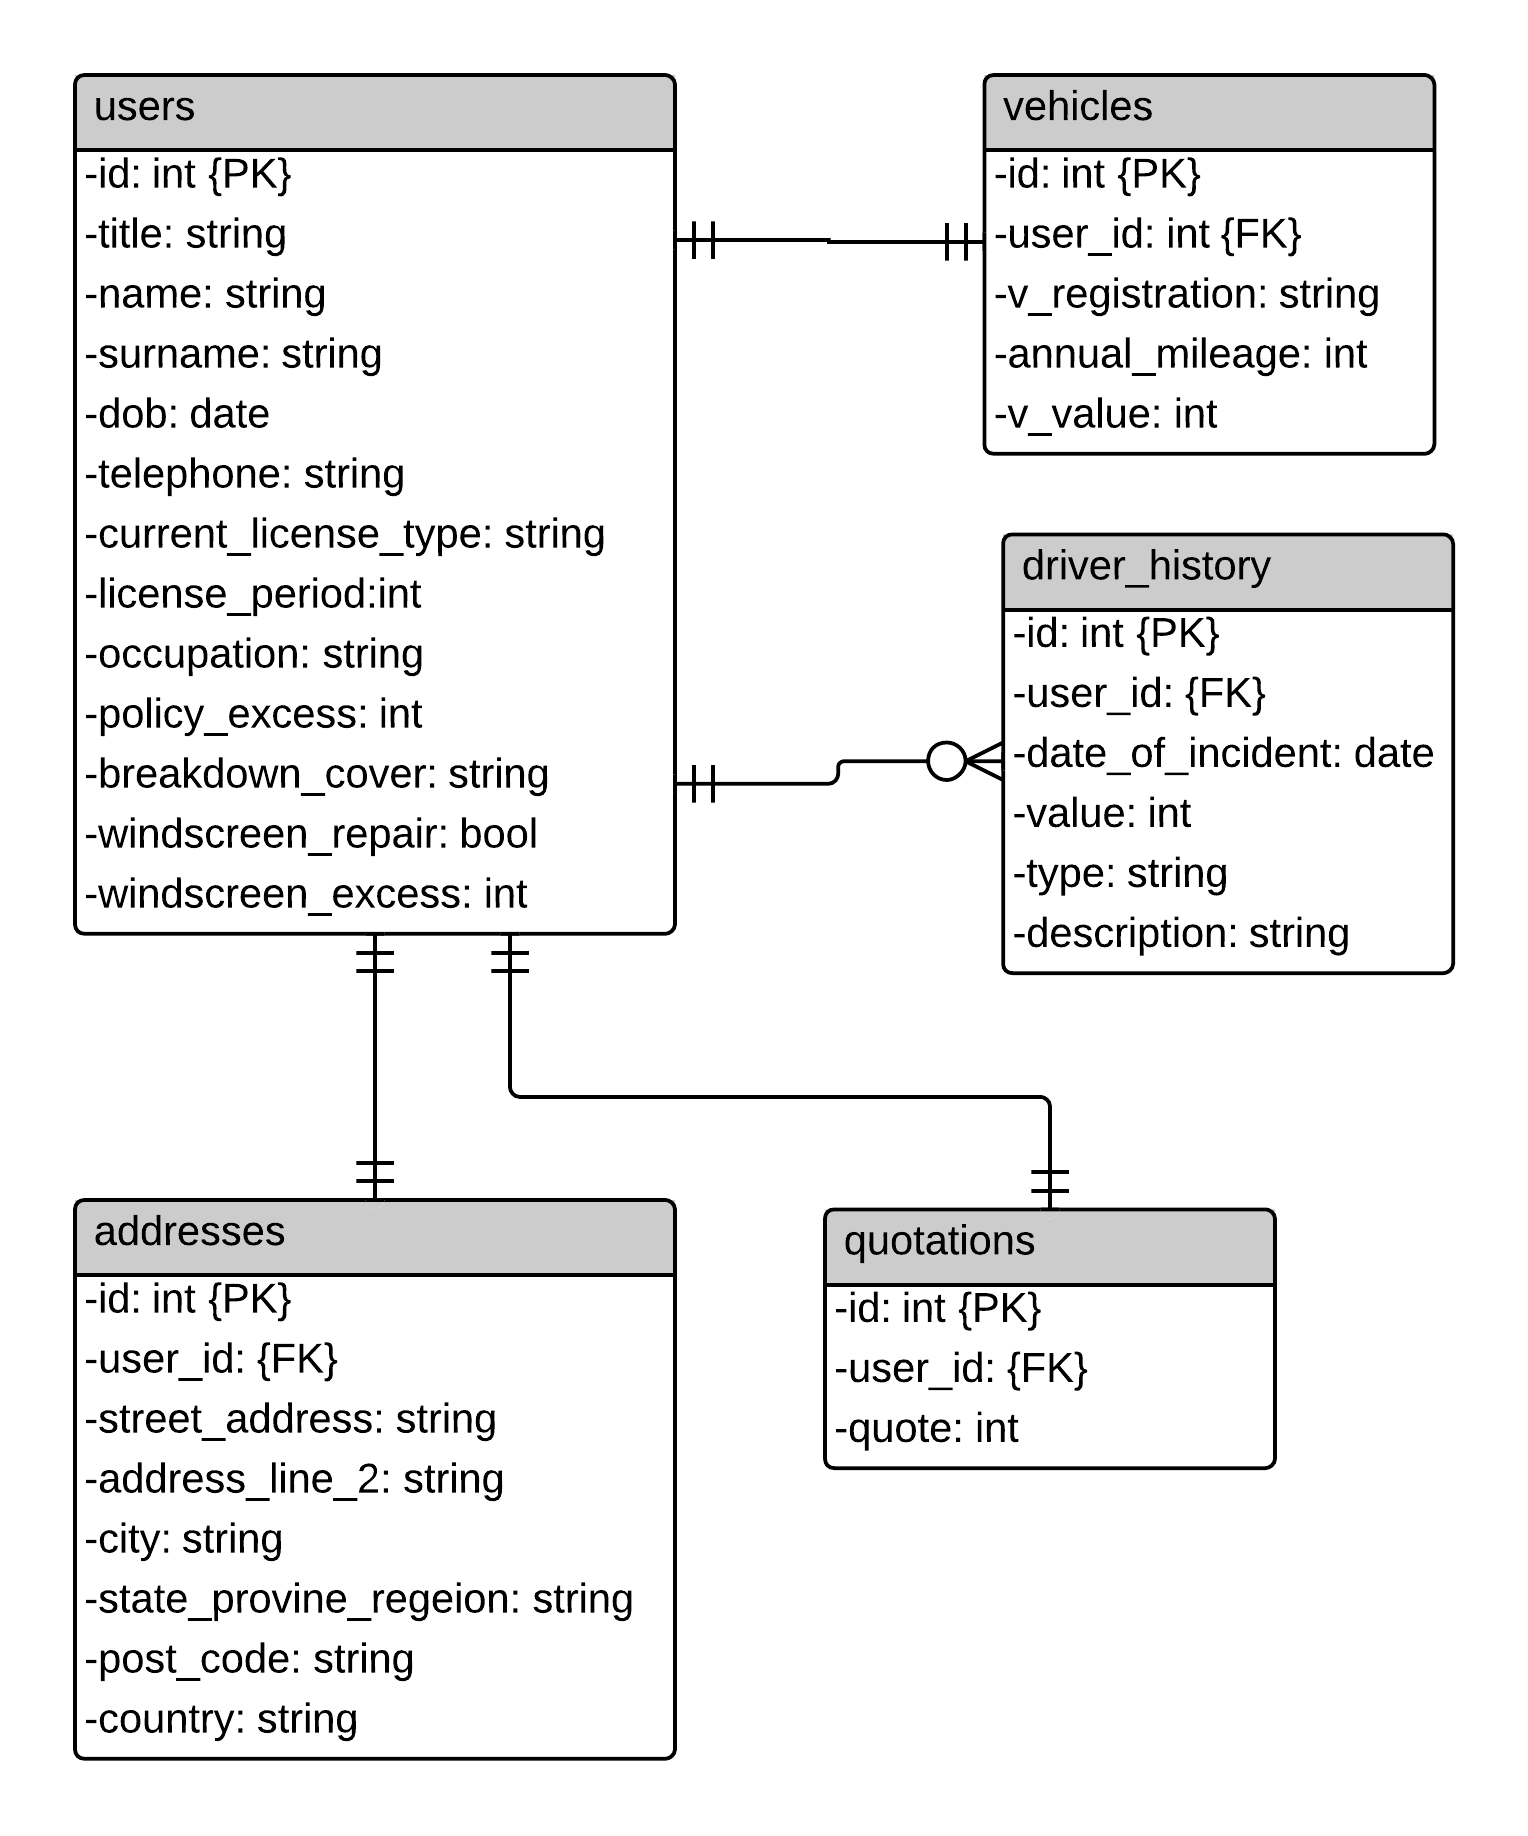
\includegraphics[scale=0.198]{./DatabaseDesign}}
\caption{Database Design}
\label{fig:DatabaseDesign}
\end{figure}

On the figure ~\ref{fig:ClassDesign} there is a class diagram of the underwriter application. The idea is to use it as a business-to-business application; instead of generating HTML pages the interaction is done using the data formatted in JSON and is expected to be used by automated clients. There is nothing under the "view" in class diagram since it only responds to the data encoded in JSON format (HTML support was left for the debugging purpose to see what is held in the database, but it would be removed in production mode). To get a quote broker submits PUT request to the \textit{/users/new.json} address with the user data, then users controller handles this request and sends back the ID assigned to the newly created user encoded as JSON. I used the ID field in "Users" table as the unique reference number for the later quote retrieval. ID fields are handled by the rails and are guaranteed to be unique across all the users: it is one of the useful ways to identify a user in the future when the quote needs to be redisplayed. Quote premium is generated by the users controller at the new user creation time and is random number in a range from the 1000 to the 5000.

\begin{figure}[H]
\centering
\centerline{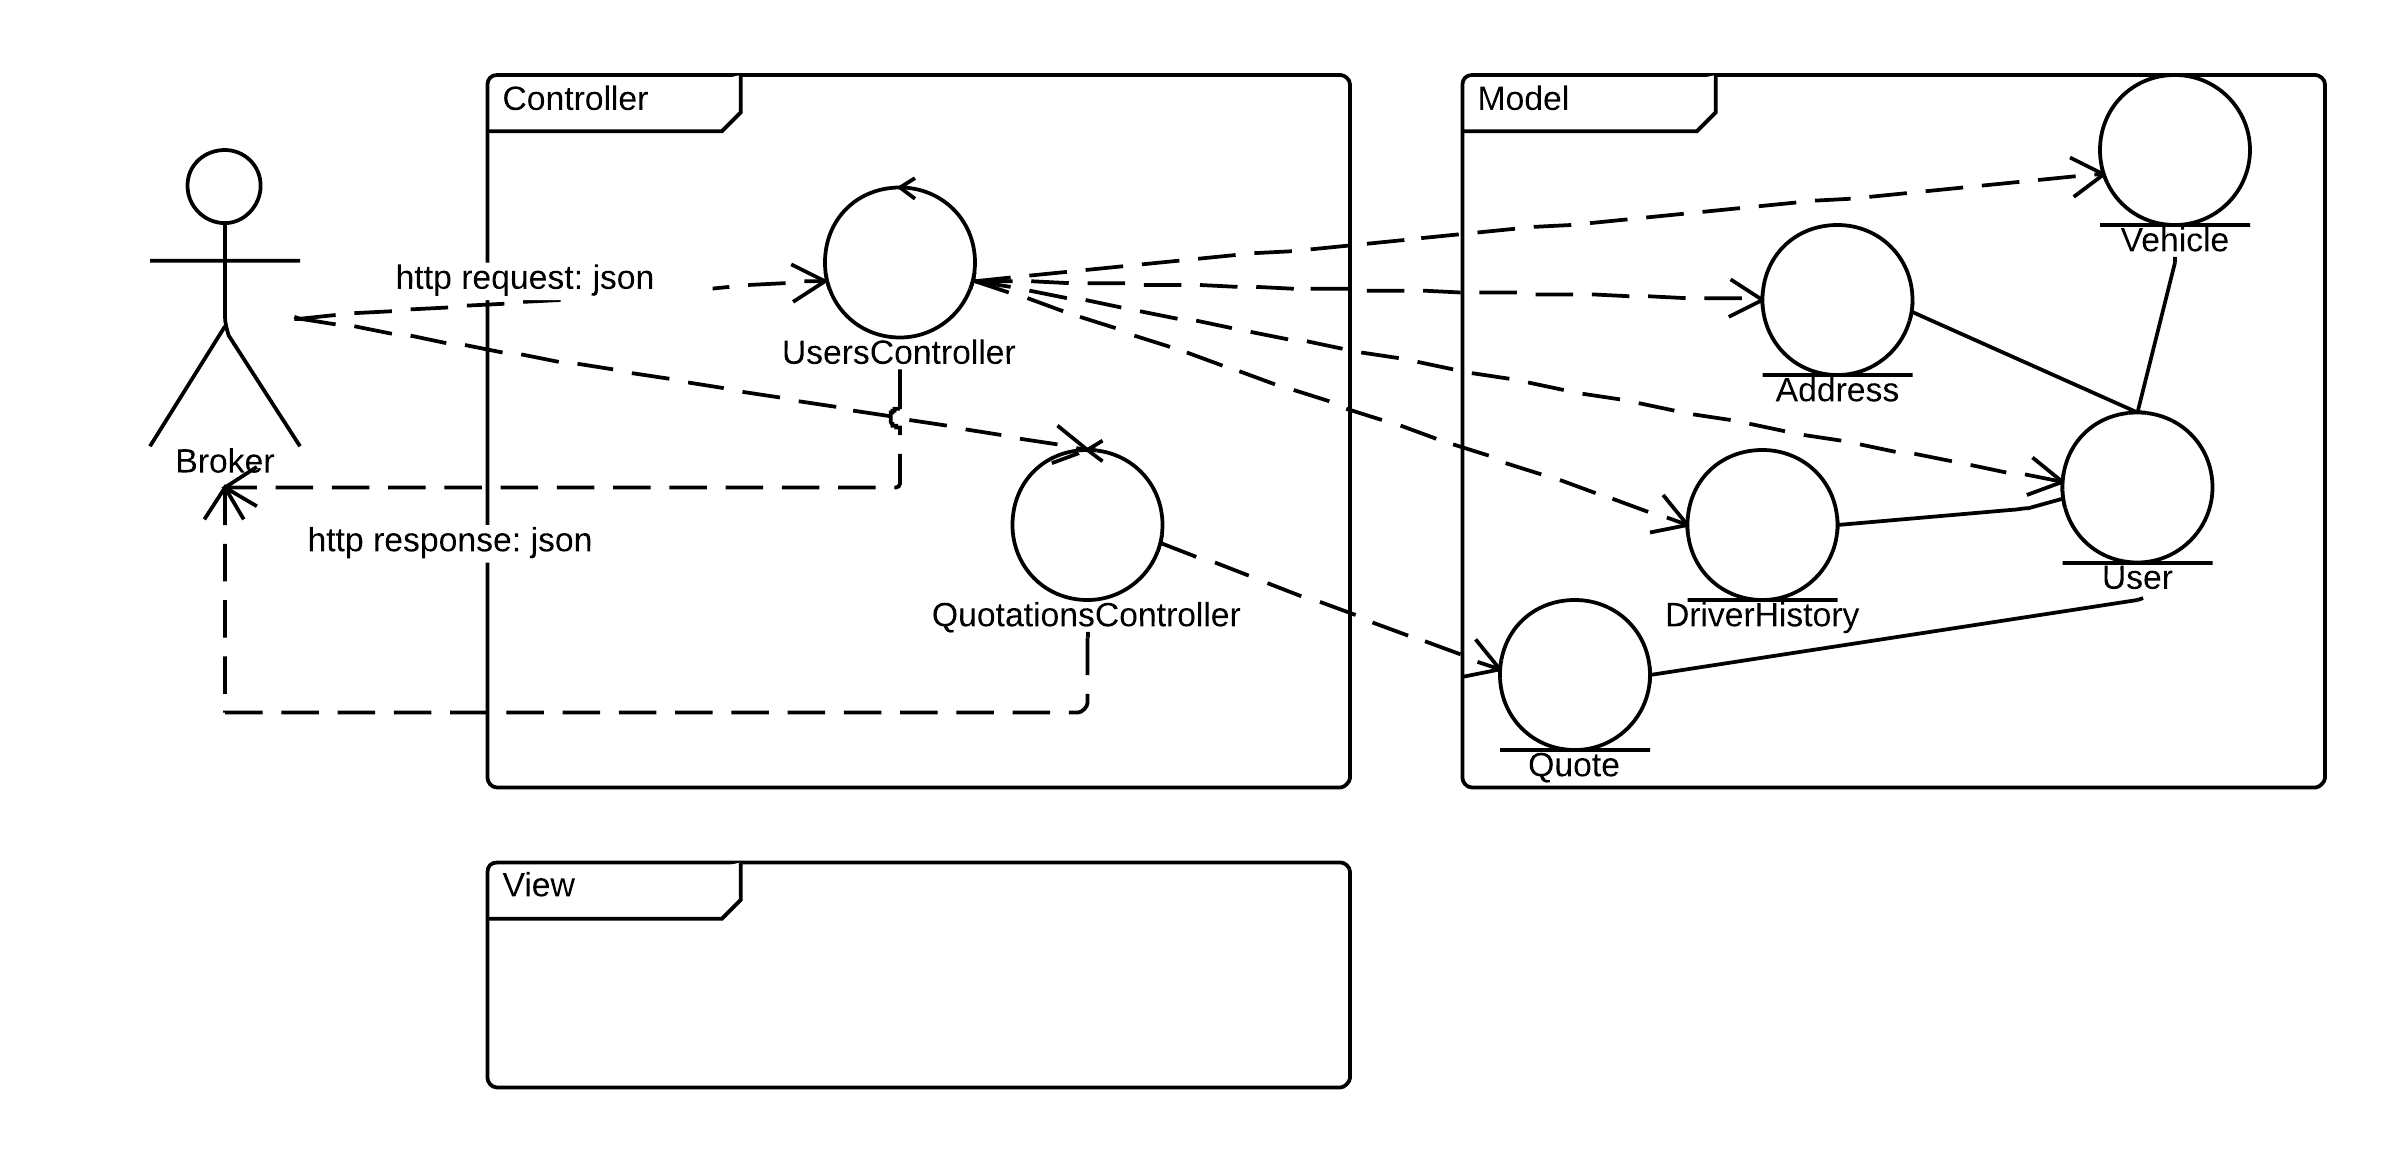
\includegraphics[scale=0.25]{./ClassDesign}}
\caption{Class Diagram}
\label{fig:ClassDesign}
\end{figure}



\section{Architecture of the RESTful broker}
The broker application was written as a web based application with the PHP support. It also uses cURL command line tool; it seems to be the only way to send JSON encoded data to the specific URL in the PHP. cURL is produced by the cURL computer software project and allows data to be transferred using various protocols \cite{cURL}. My server side scripting experience is limited to the use of SSI in HTML web pages. The fact that PHP is considered to be one of the most popular languages used for the server side coding \cite{PHP} gave me the reasons to believe that it was worth to try to use it. I had no experience in writing PHP code; this assignment was a great opportunity to make the first steps and learn to use it. The online tutorials have helped me to understand the basic concepts and start implementing my broker application.

The broker web application provides the opportunity for the potential customer to request a quote premium from the underwriter application (use case diagram is presented on the figure ~\ref{fig:usecase}). The customers interact with the broker only via HTTPS and the HTML formatted documents are transmitted to them. On the web page itself a customer needs to fill in and submit a form; on the next page a user is presented with the cost of the car insurance. This quote can be saved for the later retrieval; a customer is presented with the unique number which can be used to retrieve it. It also provides a customer with the link for a web page where the unique number can be entered and the quote will be redisplayed. The forms used on my web site were generated by the online form generator tool and modified accordingly to suite my needs. PHP is used to get the data from the forms and later on when building JSON objects containing customer data. With the help of cURL the broker application can use the standard HTTP methods to communicate with the underwrite application. To get a quotation the broker preforms the PUT request to the \textit{/users/new.json} address and receives ID number assigned to that user in the database. The broker then uses the ID received to retrieve the quotation from the underwriter using GET request and displays it to the user.

\begin{figure}[H]
\centering
\centerline{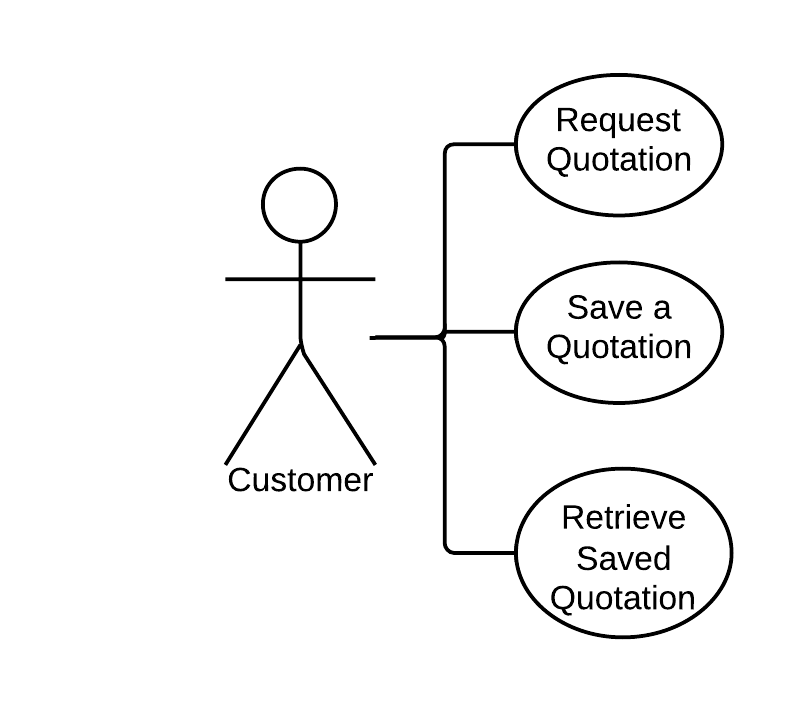
\includegraphics[scale=0.25]{./usecase}}
\caption{Use Case Diagram}
\label{fig:usecase}
\end{figure} 


\section{Test strategy}
%Write a section on your test strategy. IMPORTANT: Provide a
%screencast of your underwriter application and RESTful broker client
%working (some free screen-casting tools can be found online). This
%must focus on the broker to underwriter interworking and be no longer
%than five minutes long.

Screencast is provided on the CD; it is shown there that the broker and underwriter applications successfully communicate with each other. On the figures ~\ref{fig:brokerMain}, ~\ref{fig:quotepremium}, ~\ref{fig:QuotationNumber}, ~\ref{fig:retrivequote} and ~\ref{fig:retrievedquote} you can see screen shots taken wile testing application. There are no unit tests implemented apart from those generated by Rails.

\begin{figure}[H]
\centering
\centerline{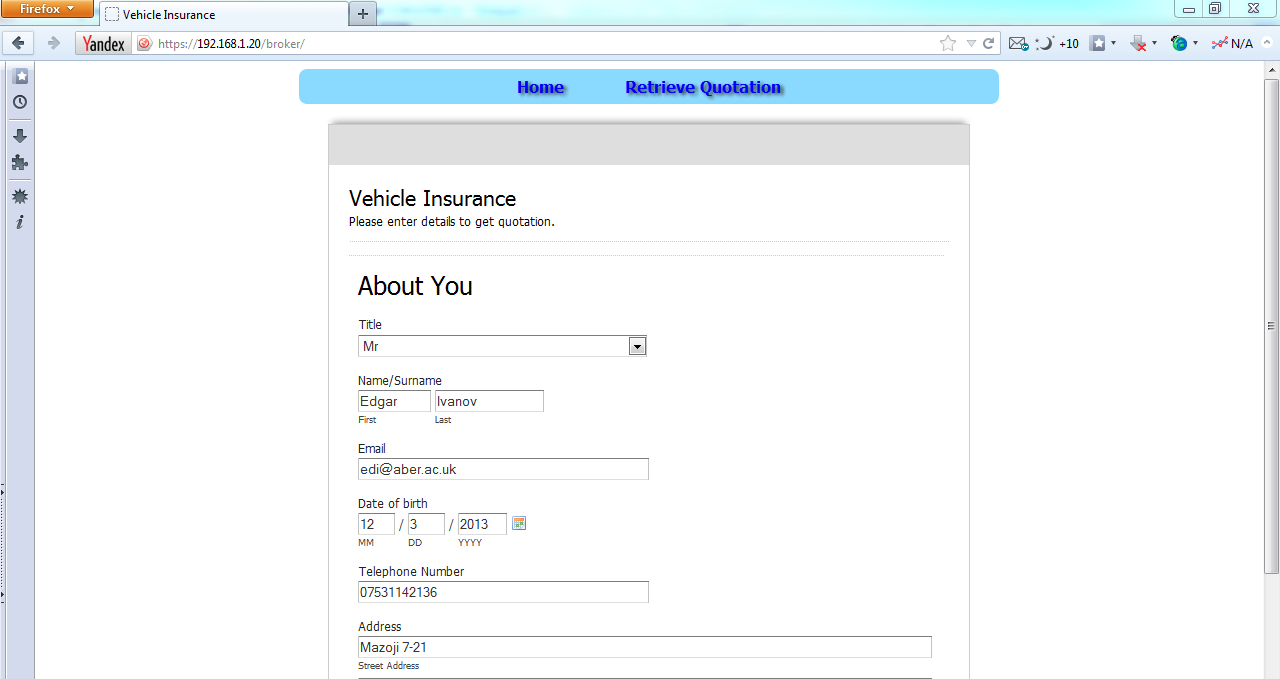
\includegraphics[scale=0.45]{./brokerMain}}
\caption{Broker Home Page}
\label{fig:brokerMain}
\end{figure} 

\begin{figure}[H]
\centering
\centerline{\includegraphics[scale=0.45]{./quotepremium}}
\caption{Quote premium displayed}
\label{fig:quotepremium}
\end{figure} 

\begin{figure}[H]
\centering
\centerline{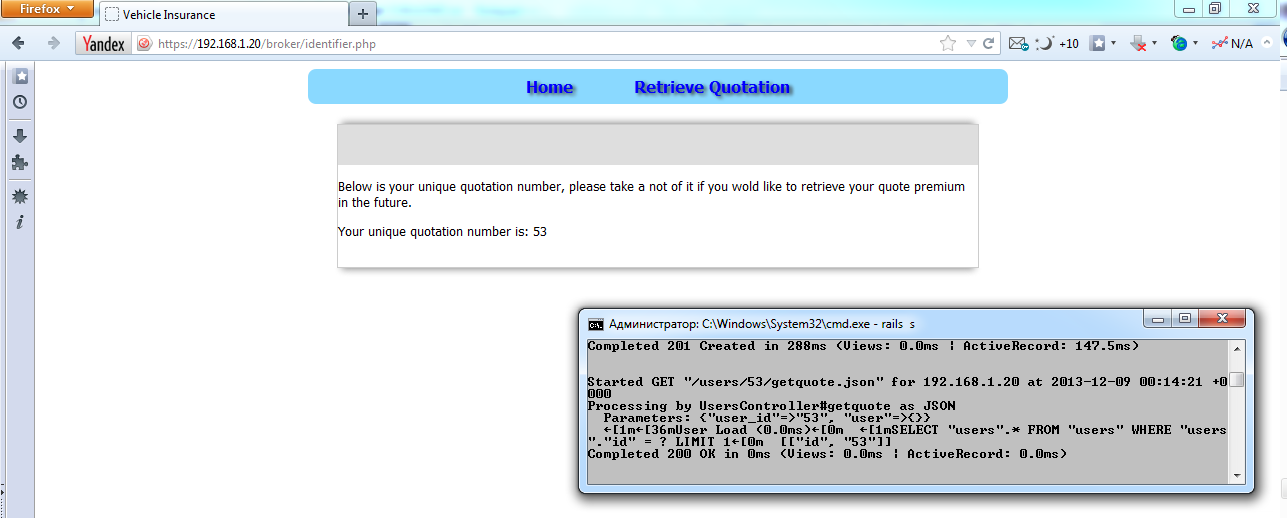
\includegraphics[scale=0.45]{./QuotationNumber}}
\caption{Quote Identifier}
\label{fig:QuotationNumber}
\end{figure}

\begin{figure}[H]
\centering
\centerline{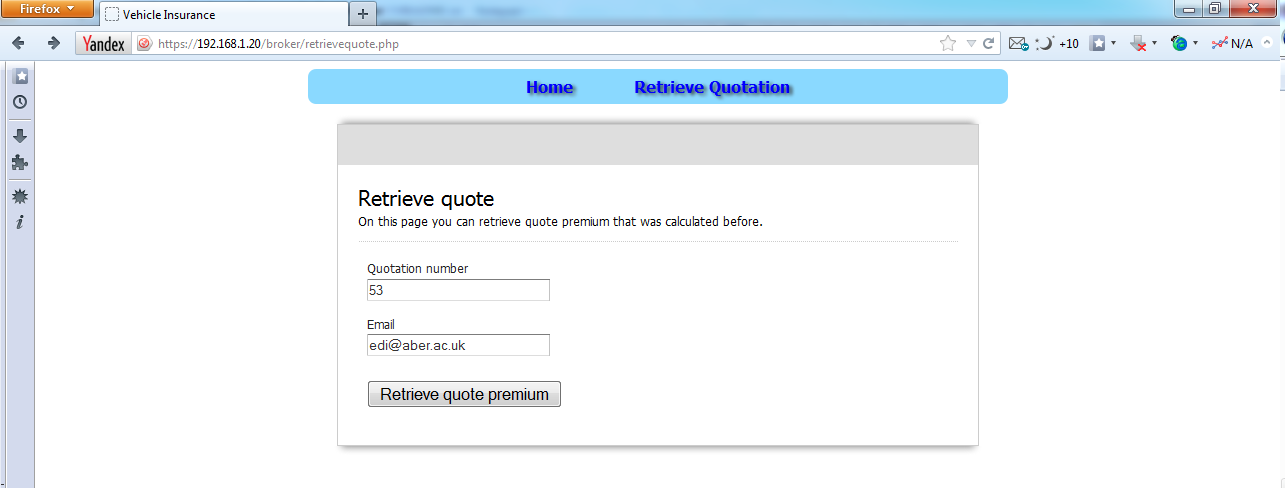
\includegraphics[scale=0.45]{./retrivequote}}
\caption{Page to retrieve quote premium}
\label{fig:retrivequote}
\end{figure} 

\begin{figure}[H]
\centering
\centerline{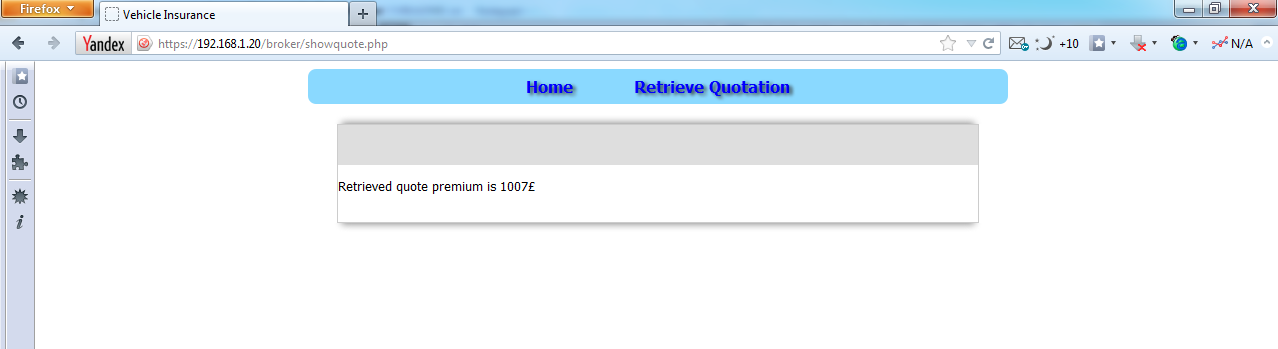
\includegraphics[scale=0.45]{./retrievedquote}}
\caption{Retrieved quote premium}
\label{fig:retrievedquote}
\end{figure} 

Table ~\ref{fig:testing} presents results of carried testing. 

\begin{center}
\begin{table}


\begin{tabularx}{\textwidth} { |p{0.14cm}|p{0.88cm}|X|X|X|p{0.6cm}|X|}
   \hline                        
  ID &  Require ment & Description &  Inputs  &  Expected outputs & Pass/ Fail & Comments  \\ \hline
   1 & FR1 &  Request a quotation & Standard user details are entered &  Display page with quote premium & P &  \\ \hline
   2 & FR2 & Save a Quotation & "Get quote identifier" button is clicked &  Display page with unique identifier & P &  \\ \hline
   3 & FR3 & Retrieve a Saved Quotation & Identifier and user email are entered &  Redisplay page with quote premium & P & \\ \hline
   4 & Show error if car value is 0 & When user enters 0 in the car value field, system should display an error &  Car value = 0 &  Display message explaining that car value cannot be 0 & F & System treats value as normal and returns quote premium\\ \hline
   5 & Show error if email address is not valid & If user has wrong characters in the email address field error should be displayed& email = edi\#aber,ac.uk &  Display message that email contains wrong characters & F & System doesn't have any validators to check if email is in a right form and returns quote premium\\ \hline
   6 & Show additional fields for each incident & Web site should generate additional form with fields for each incident& Number of incidents = 5  &  Additional form is shown to enter information about five incidents & F & This feature is not implemented in the system\\ \hline
   7 & Display message if quotation identifier is wrong&  If user enters enters quotation identifier that doesn't exist in the database error message should be shown  &Quotation number = 54  &  Display message that user quote for this user couldn't be found & F & No validation implemented, broker system displays response from the Rails, figure ~\ref{fig:retriveQuoteError}\\ \hline
   8 & Presence of information in all fields &  Validates that user filled in all fields in the form &  Submit blank form & Error message indicating that all fields form should be completed & F & Broker displays message returned by the underwriter, it is possible for technical person to understand what went wrong but ideal solution would handle such situation and display more user-friendly message \\ \hline
   
   
   \hline  
   
\end{tabularx}
\caption{Test table}
\label{fig:testing}
\end{table}
\end{center}


\begin{figure}[H]
\centering
\centerline{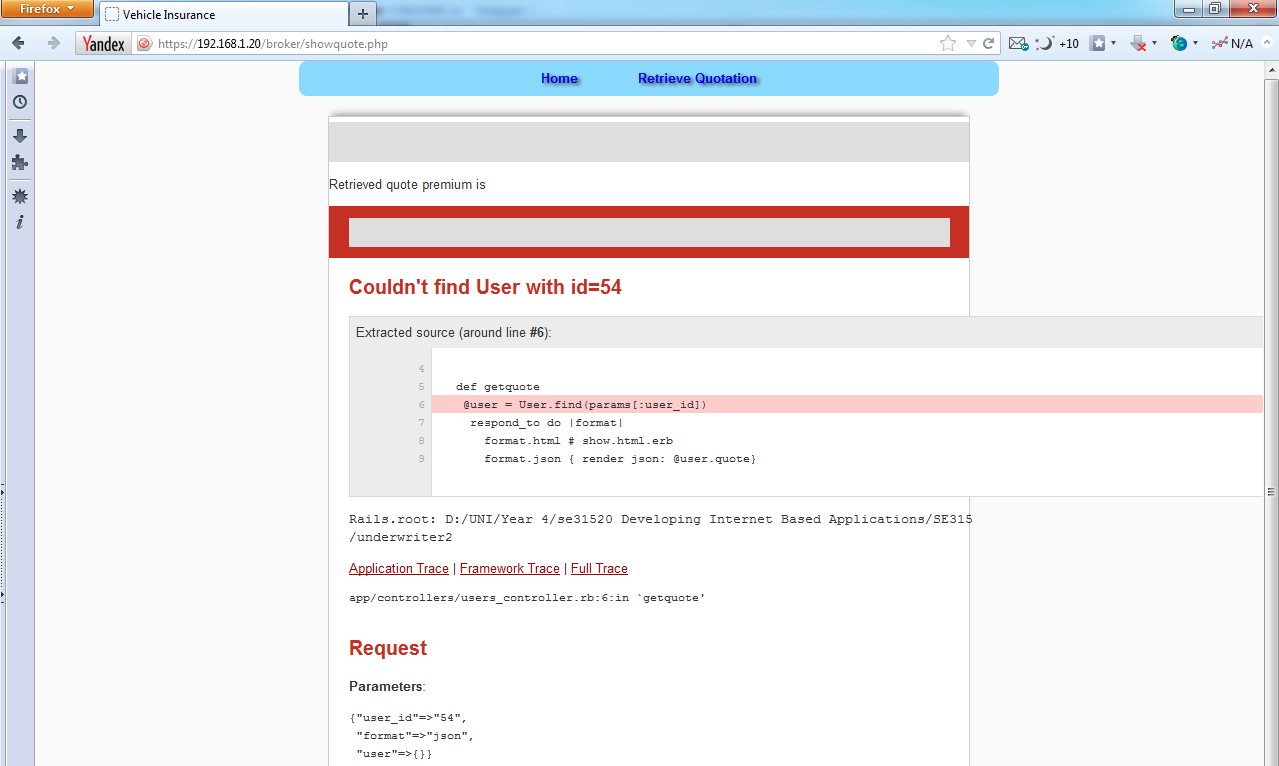
\includegraphics[scale=0.45]{./retriveQuoteError}}
\caption{Error when retrieving quote for non-existent user}
\label{fig:retriveQuoteError}
\end{figure} 
\newpage
\section{Self-evaluation}
Mark to be awarded 50-60. My resultant system, although not ideal, works. Underwriter side is built as a RESTful web service using ROR and can be communicated using standard HTTP methods with JSON objects used for the representational state transfer as required by the assignment. The broker application is represented by a web site and is accessible throughout the Internet browsers; it supports HTTPS for the communication - it means that the data sent between the customer and the broker is secure.

In the beginning it was challenging to understand how ROR worked. Adding one line of code in one place would completely change application behaviour in the other. It took me some time to understand how to use routes.rb file and the fact that I should expose my methods to the world in the controller throughout this file as well. It took me over two weeks to figure out little things in the ROR that make everything function. I experienced problems when trying to use XML to make both applications to interact with each other, but later on I found out that scaffold generator generated the code for CRUD operations that has support for the JSON format already. Initially I spent too much time trying to build the support for the CRUD operations and database migration files by myself instead of using Rails scaffold generator originally, which did the job for me later on. Although my class diagram in the "Architecture of the underwriter" section contains models for the addresses, vehicle information, quotes and driver history I didn't implement them in the resultant system. Instead all the customer's information is in the "Users" table and is managed by the users controller; that is clearly not an ideal solution. While working on this assignment I gained a lot of new knowledge: I understood how MVC pattern was applied and worked in the real world, I started to learn PHP and Ruby programming languages as well as Rails web application framework which makes a process of building a web site easier.

\subsection{Conclusion}
This assignment was interesting and very challenging; it required the use and understanding of the different technologies like web server software, use of HTTPS for secure communication, PHP and cURL for server side scripting, ROR for building RESTful web service, understanding of MVC patter and use of relational database management system. In the middle of the work, when I understood how ROR worked, what RESTful really meant and how to interconnect two systems I have started to enjoy the process and dig deeper to gain more knowledge of all the elements involved.  

%Write a self-evaluation section. Say what mark you should be awarded
%and why. Say what you found hard or easy, and what was omitted and
%why. Provide an analysis of your design and the appropriateness, or
%otherwise, of the technologies used.

\bibliographystyle{ieeetr}
\bibliography{bibl}

\end{document}